\documentclass[12pt,letterpaper]{article}

% =========================
% PAQUETES
% =========================
\usepackage[spanish,es-tabla]{babel}
\usepackage[utf8]{inputenc}
\usepackage[T1]{fontenc}
\usepackage{lmodern}
\usepackage{geometry}
\usepackage{setspace}
\usepackage{graphicx}
\usepackage{float}
\usepackage{booktabs}
\usepackage{array}
\usepackage{amsmath}
\usepackage{amssymb}
\usepackage{hyperref}
\usepackage{xcolor}
\usepackage{listings}
\usepackage{caption}
\usepackage{longtable}

% =========================
% CONFIGURACIÓN GENERAL
% =========================
\geometry{
    left=2.5cm,
    right=2.5cm,
    top=2.5cm,
    bottom=2.5cm
}

\onehalfspacing
\setlength{\parindent}{0pt}
\setlength{\parskip}{6pt}

\graphicspath{{img/}}

\hypersetup{
    colorlinks=true,
    linkcolor=black,
    urlcolor=blue,
    citecolor=black
}

\lstset{
    basicstyle=\ttfamily\small,
    breaklines=true,
    frame=single,
    numbers=left,
    numberstyle=\tiny,
    keywordstyle=\color{blue},
    commentstyle=\color{gray},
    stringstyle=\color{red},
    tabsize=4,
    showstringspaces=false
}

% =========================
% PORTADA
% =========================
\title{
    \textbf{Práctica 1: Optimización de Código}\\
    \large Asignatura Tópicos A
}

\author{
    Luis Antonio Muñoz Vásquez\\
    Universidad de Magallanes
}

\date{Mayo de 2026}

\begin{document}

\maketitle
\thispagestyle{empty}

\vspace{1cm}

\begin{center}
    \textbf{Facultad de Ingeniería}\\
    Departamento de Ingeniería en Computación
\end{center}

\vfill

\begin{center}
    Punta Arenas, Chile
\end{center}

\newpage

\tableofcontents
\newpage

% =========================
% INTRODUCCIÓN
% =========================
\section{Introducción}

La presente práctica tiene como finalidad estudiar el rendimiento computacional de distintas operaciones de álgebra lineal, comparando implementaciones realizadas en GNU Octave, lenguaje C y funciones de la biblioteca CBLAS.

Las operaciones evaluadas fueron el producto punto, la multiplicación matriz-vector y la multiplicación matriz-matriz. Estas operaciones fueron seleccionadas debido a que representan distintos órdenes de complejidad algorítmica: lineal, cuadrático y cúbico, respectivamente.

El trabajo se desarrolló en un entorno WSL, utilizando herramientas de compilación y medición como GCC, Octave, CBLAS, Bash y Gnuplot. Se implementaron versiones manuales en C, versiones optimizadas y se compararon con rutinas especializadas de CBLAS.

El objetivo central fue observar cómo influyen la complejidad algorítmica, el tipo de lenguaje, la optimización de código y la localidad de memoria sobre los tiempos de ejecución.

% =========================
% OBJETIVOS
% =========================
\section{Objetivos}

\subsection{Objetivo general}

Comparar el rendimiento de operaciones de álgebra lineal implementadas en Octave, C manual, C optimizado y CBLAS, evaluando el efecto de la complejidad algorítmica y de las técnicas de optimización de código.

\subsection{Objetivos específicos}

\begin{itemize}
    \item Implementar y medir el tiempo de ejecución del producto punto, multiplicación matriz-vector y multiplicación matriz-matriz.
    \item Comparar operadores nativos de Octave con implementaciones propias.
    \item Implementar las mismas operaciones en lenguaje C.
    \item Aplicar técnicas de optimización como loop unrolling y cambio de orden de ciclos.
    \item Comparar las implementaciones manuales y optimizadas con funciones CBLAS.
    \item Analizar los resultados obtenidos a partir de tablas y gráficas.
\end{itemize}

% =========================
% MARCO TEÓRICO
% =========================
\section{Marco teórico}

\subsection{Complejidad algorítmica}

La complejidad algorítmica permite estudiar cómo crece el costo computacional de un algoritmo a medida que aumenta el tamaño del problema. En esta práctica se analizaron tres operaciones fundamentales.

\subsubsection{Producto punto}

El producto punto entre dos vectores de tamaño $n$ se define como:

\begin{equation}
    c = \sum_{i=1}^{n} x_i y_i
\end{equation}

La operación requiere recorrer los vectores una vez, por lo que su complejidad es:

\begin{equation}
    O(n)
\end{equation}

\subsubsection{Multiplicación matriz-vector}

La multiplicación entre una matriz $A \in \mathbb{R}^{n \times n}$ y un vector $x \in \mathbb{R}^{n}$ se define como:

\begin{equation}
    y_i = \sum_{j=1}^{n} A_{ij}x_j
\end{equation}

Esta operación requiere dos ciclos anidados, por lo que su complejidad es:

\begin{equation}
    O(n^2)
\end{equation}

\subsubsection{Multiplicación matriz-matriz}

La multiplicación entre dos matrices cuadradas $A$ y $B$ de tamaño $n \times n$ se define como:

\begin{equation}
    C_{ij} = \sum_{k=1}^{n} A_{ik}B_{kj}
\end{equation}

Esta operación requiere tres ciclos anidados, por lo que su complejidad es:

\begin{equation}
    O(n^3)
\end{equation}

\subsection{GNU Octave}

GNU Octave permite resolver operaciones de álgebra lineal mediante operadores nativos. Estos operadores suelen estar asociados a rutinas compiladas y optimizadas, por lo que pueden presentar tiempos de ejecución considerablemente menores que una función escrita directamente en Octave mediante ciclos interpretados.

\subsection{CBLAS}

CBLAS corresponde a una interfaz en lenguaje C para acceder a rutinas BLAS. Estas rutinas están diseñadas para operaciones de álgebra lineal y suelen estar altamente optimizadas.

En esta práctica se utilizaron las siguientes funciones:

\begin{itemize}
    \item \texttt{cblas\_ddot}: producto punto.
    \item \texttt{cblas\_dgemv}: multiplicación matriz-vector.
    \item \texttt{cblas\_dgemm}: multiplicación matriz-matriz.
\end{itemize}

\subsection{Optimización de código}

La optimización de código busca reducir el tiempo de ejecución de un programa sin modificar el resultado final. En esta práctica se aplicaron dos estrategias principales:

\begin{itemize}
    \item \textbf{Loop unrolling}: técnica que reduce la sobrecarga de control de ciclos, realizando varias operaciones por iteración.
    \item \textbf{Cambio de orden de ciclos}: técnica orientada a mejorar el acceso a memoria y la localidad de datos, especialmente relevante en operaciones con matrices.
\end{itemize}

% =========================
% METODOLOGÍA
% =========================
\section{Metodología}

\subsection{Entorno de trabajo}

El desarrollo se realizó en WSL utilizando las siguientes herramientas:

\begin{itemize}
    \item GNU Octave para implementar y medir operaciones interpretadas.
    \item GCC para compilar programas en C.
    \item CBLAS mediante la biblioteca \texttt{libblas-dev}.
    \item Bash para automatizar las mediciones.
    \item Gnuplot para generar las gráficas.
    \item LaTeX para elaborar el informe.
\end{itemize}

\subsection{Procedimiento de medición}

Para cada tamaño del problema se ejecutó cada algoritmo siete veces. Luego, se calculó el promedio de los tiempos obtenidos. Esta estrategia permite reducir el efecto de variaciones puntuales del sistema operativo o de la carga de CPU.

En Octave se utilizaron las funciones \texttt{tic} y \texttt{toc}. En C se utilizó la función \texttt{gettimeofday}. Los datos fueron almacenados en archivos \texttt{.dat} y posteriormente graficados con Gnuplot.

\subsection{Tamaños utilizados}

Los tamaños de entrada fueron seleccionados de forma progresiva, usando potencias de dos. Se buscó alcanzar tiempos mayores a $0.01$ segundos, ya que tiempos demasiado pequeños pueden producir mediciones poco confiables.

% =========================
% IMPLEMENTACIONES
% =========================
\section{Implementaciones}

\subsection{Producto punto}

Para el producto punto se implementaron las siguientes versiones:

\begin{itemize}
    \item Función manual en Octave.
    \item Operador nativo de Octave.
    \item Implementación manual en C.
    \item Implementación optimizada en C mediante loop unrolling.
    \item Función \texttt{cblas\_ddot}.
\end{itemize}

La versión manual en C utiliza un ciclo simple:

\begin{lstlisting}[language=C]
for(i = 0; i < n; i++)
    c += x[i] * y[i];
\end{lstlisting}

La versión optimizada realiza varias operaciones dentro de una misma iteración:

\begin{lstlisting}[language=C]
for(i = 0; i < limit; i += 5)
{
    c += x[i] * y[i]
       + x[i + 1] * y[i + 1]
       + x[i + 2] * y[i + 2]
       + x[i + 3] * y[i + 3]
       + x[i + 4] * y[i + 4];
}
\end{lstlisting}

\subsection{Multiplicación matriz-vector}

La implementación manual de matriz-vector utiliza dos ciclos anidados:

\begin{lstlisting}[language=C]
for(i = 0; i < m; i++)
{
    y[i] = 0.0;
    for(j = 0; j < n; j++)
    {
        y[i] += A[i * n + j] * x[j];
    }
}
\end{lstlisting}

La versión optimizada utiliza un acumulador local y loop unrolling en el ciclo interno, disminuyendo accesos innecesarios a memoria.

\subsection{Multiplicación matriz-matriz}

La implementación manual se realizó mediante tres ciclos anidados en el orden clásico:

\begin{lstlisting}[language=C]
for(i = 0; i < m; i++)
{
    for(j = 0; j < n; j++)
    {
        double sum = 0.0;
        for(p = 0; p < k; p++)
        {
            sum += A[i * k + p] * B[p * n + j];
        }
        C[i * n + j] = sum;
    }
}
\end{lstlisting}

La versión optimizada utiliza el orden de ciclos $i$, $p$, $j$, lo que permite recorrer de forma más contigua la matriz $B$ y la matriz $C$ en memoria:

\begin{lstlisting}[language=C]
for(i = 0; i < m; i++)
{
    for(p = 0; p < k; p++)
    {
        double a_ip = A[i * k + p];
        int rowB = p * n;
        int rowC = i * n;

        for(j = 0; j < n; j++)
        {
            C[rowC + j] += a_ip * B[rowB + j];
        }
    }
}
\end{lstlisting}

% =========================
% RESULTADOS
% =========================
\section{Resultados}

\subsection{Resultados en Octave}

\subsubsection{Producto punto en Octave}

\begin{figure}[H]
    \centering
    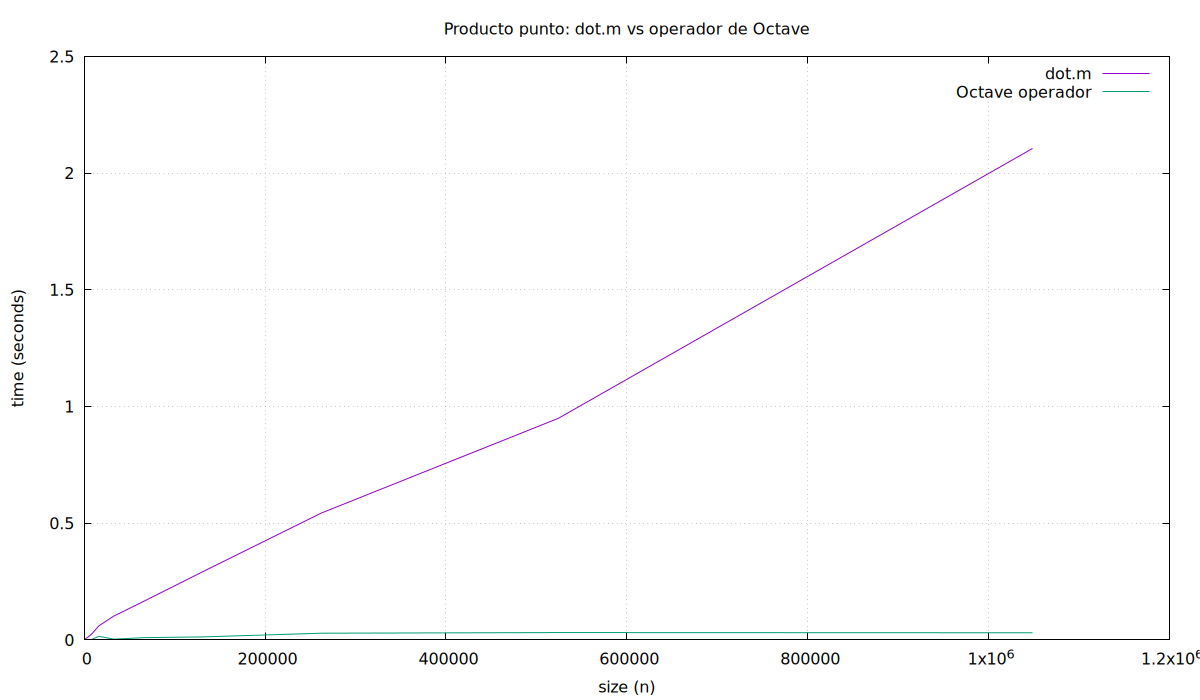
\includegraphics[width=0.9\textwidth]{octave_dot.png}
    \caption{Comparación del producto punto implementado en Octave y operador nativo.}
    \label{fig:octave_dot}
\end{figure}

\subsubsection{Multiplicación matriz-vector en Octave}

\begin{figure}[H]
    \centering
    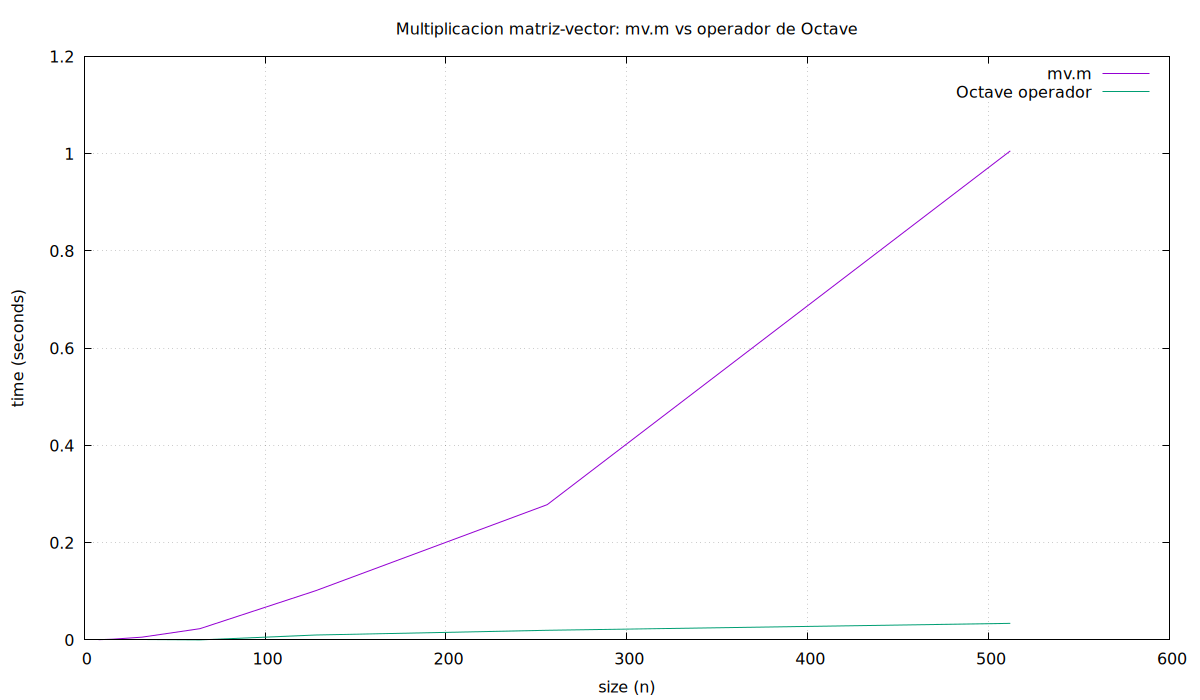
\includegraphics[width=0.9\textwidth]{octave_mv.png}
    \caption{Comparación de multiplicación matriz-vector implementada en Octave y operador nativo.}
    \label{fig:octave_mv}
\end{figure}

\subsubsection{Multiplicación matriz-matriz en Octave}

\begin{figure}[H]
    \centering
    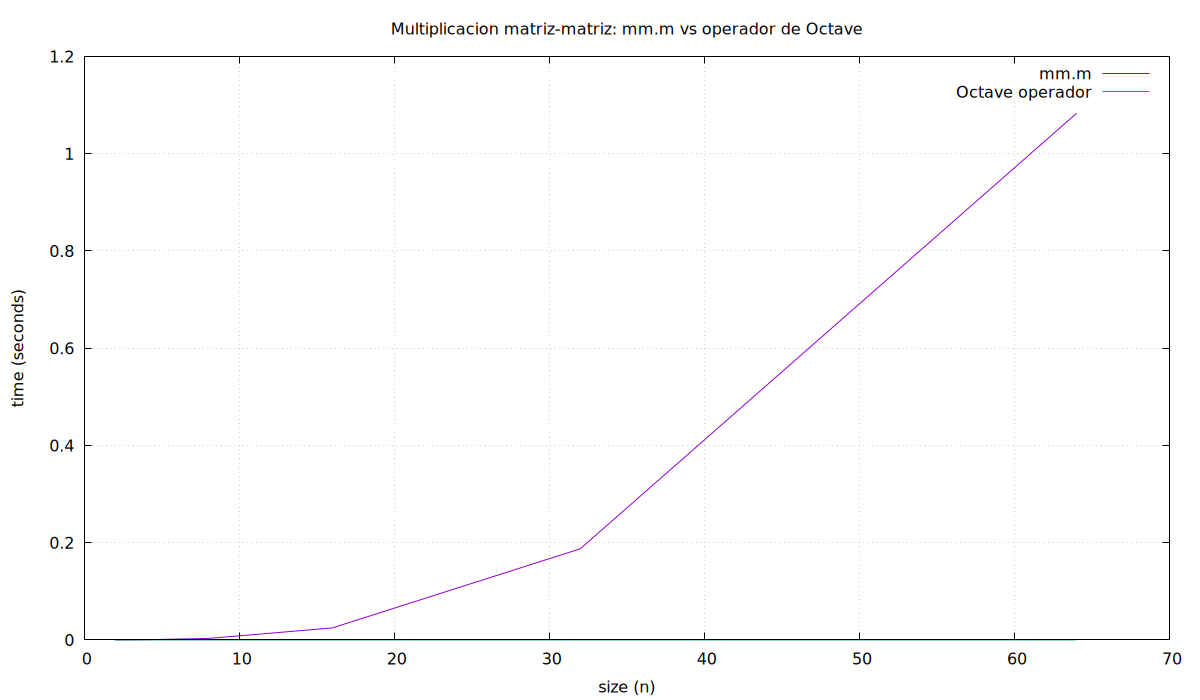
\includegraphics[width=0.9\textwidth]{octave_mm.png}
    \caption{Comparación de multiplicación matriz-matriz implementada en Octave y operador nativo.}
    \label{fig:octave_mm}
\end{figure}

\subsection{Resultados con CBLAS}

\subsubsection{Producto punto con \texttt{cblas\_ddot}}

\begin{figure}[H]
    \centering
    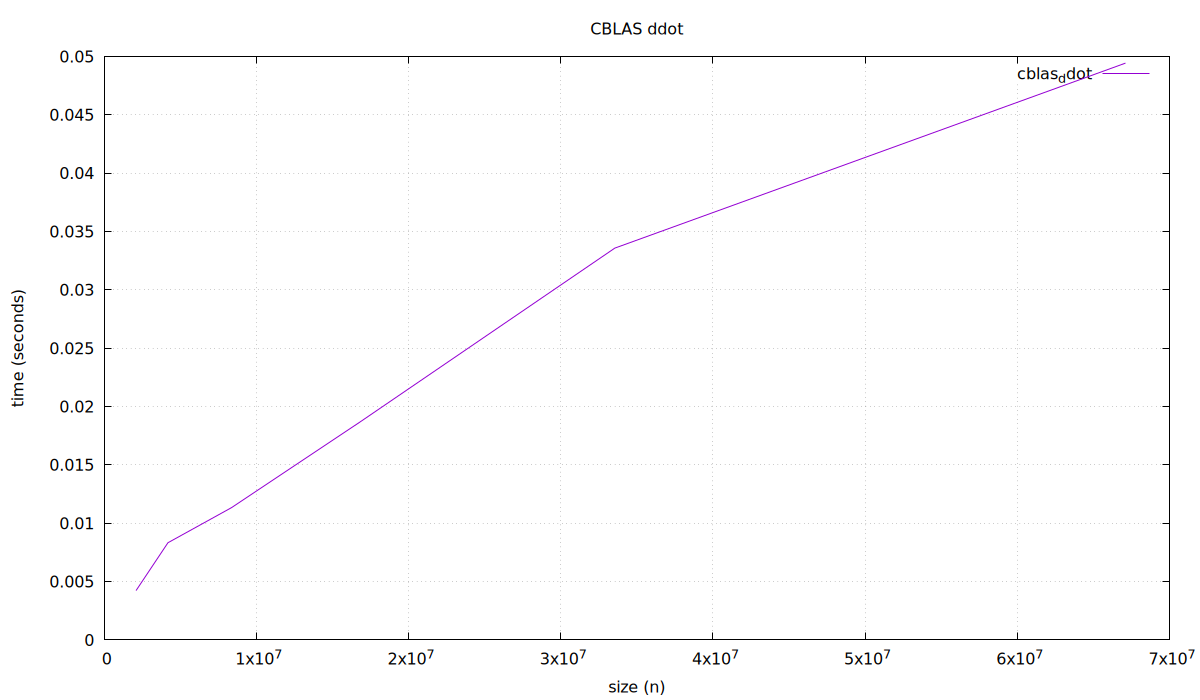
\includegraphics[width=0.9\textwidth]{cblas_ddot.png}
    \caption{Tiempo de ejecución de \texttt{cblas\_ddot}.}
    \label{fig:cblas_ddot}
\end{figure}

\subsubsection{Multiplicación matriz-vector con \texttt{cblas\_dgemv}}

\begin{figure}[H]
    \centering
    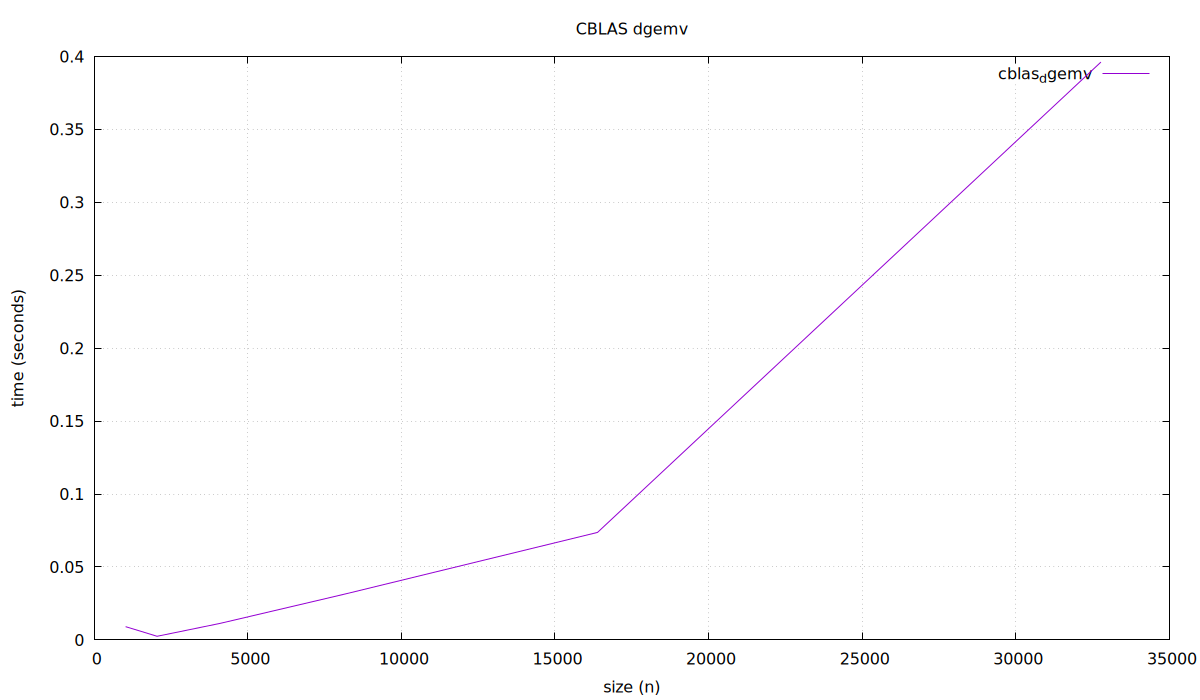
\includegraphics[width=0.9\textwidth]{cblas_dgemv.png}
    \caption{Tiempo de ejecución de \texttt{cblas\_dgemv}.}
    \label{fig:cblas_dgemv}
\end{figure}

\subsubsection{Multiplicación matriz-matriz con \texttt{cblas\_dgemm}}

\begin{figure}[H]
    \centering
    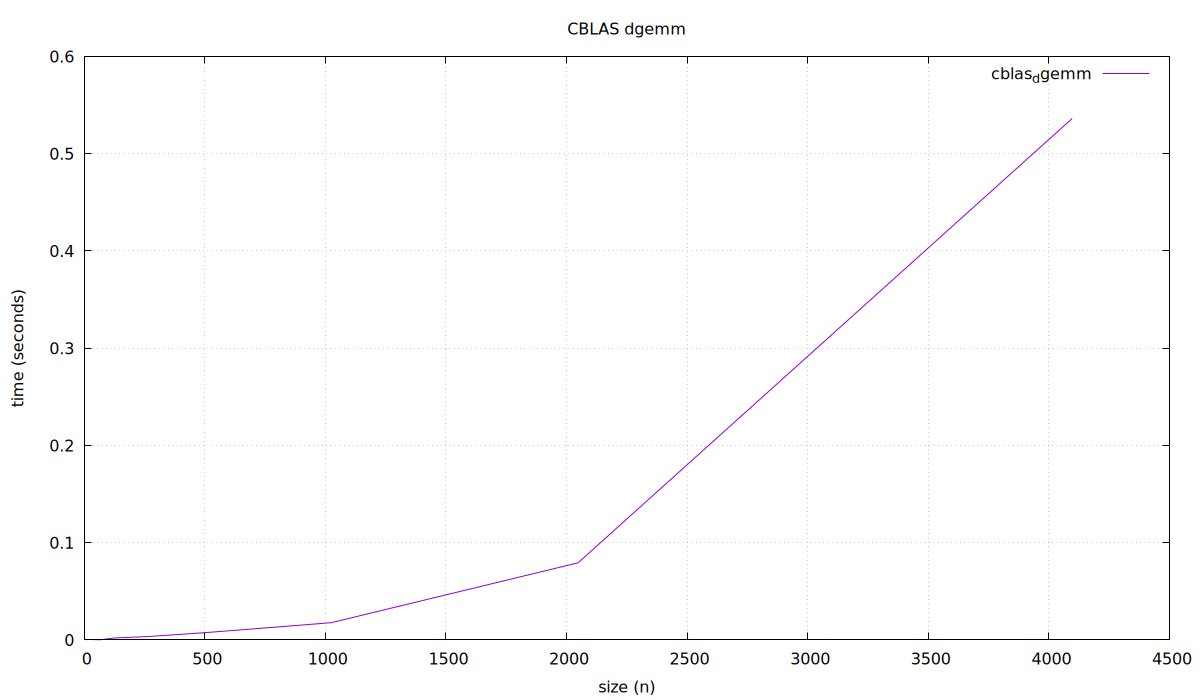
\includegraphics[width=0.9\textwidth]{cblas_dgemm.png}
    \caption{Tiempo de ejecución de \texttt{cblas\_dgemm}.}
    \label{fig:cblas_dgemm}
\end{figure}

\subsection{Comparación C manual, C optimizado y CBLAS}

\subsubsection{Producto punto}

\begin{table}[H]
\centering
\caption{Tiempos de ejecución para producto punto.}
\begin{tabular}{rrrr}
\toprule
$n$ & C manual & C optimizado & CBLAS \\
\midrule
2097152 & 0.00197586 & 0.00169957 & 0.00213343 \\
4194304 & 0.00422486 & 0.00346971 & 0.00475314 \\
8388608 & 0.00798214 & 0.00614800 & 0.00580186 \\
16777216 & 0.01624690 & 0.01267610 & 0.00743729 \\
33554432 & 0.03522290 & 0.02433260 & 0.01515530 \\
67108864 & 0.06923540 & 0.04843470 & 0.02964730 \\
\bottomrule
\end{tabular}
\end{table}

\begin{figure}[H]
    \centering
    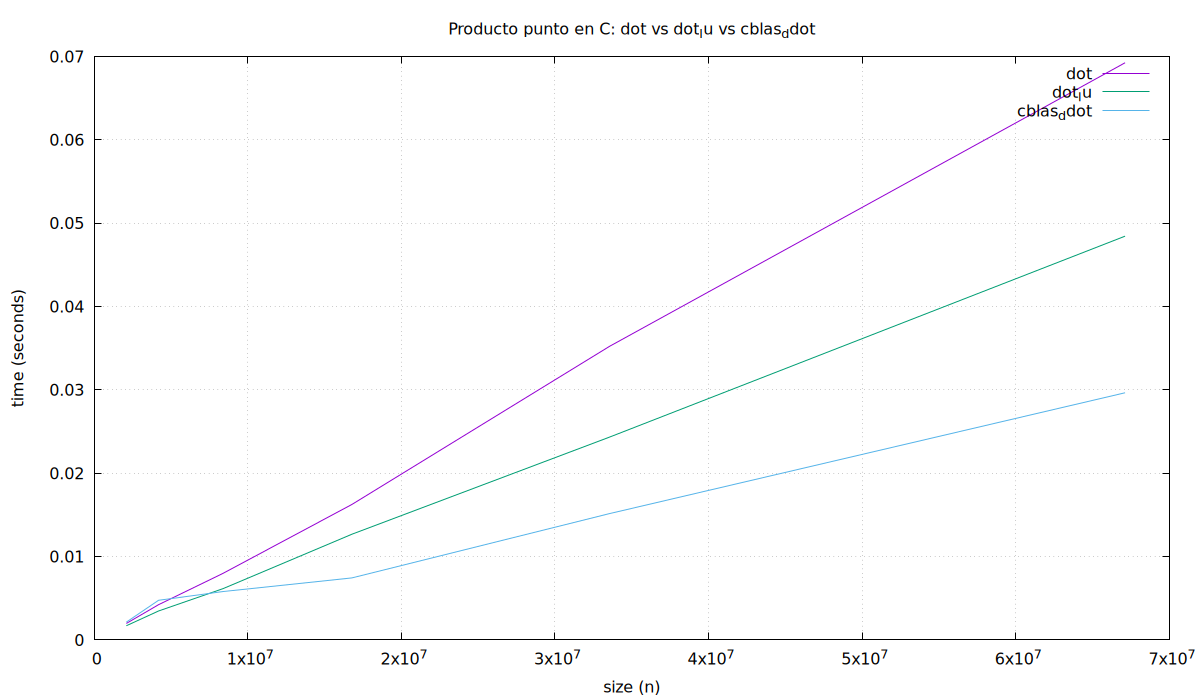
\includegraphics[width=0.9\textwidth]{c_dot_compare.png}
    \caption{Comparación entre producto punto manual, optimizado y CBLAS.}
    \label{fig:c_dot_compare}
\end{figure}

\subsubsection{Multiplicación matriz-vector}

\begin{table}[H]
\centering
\caption{Tiempos de ejecución para multiplicación matriz-vector.}
\begin{tabular}{rrrr}
\toprule
$n$ & C manual & C optimizado & CBLAS \\
\midrule
1024 & 0.00102200 & 0.00067200 & 0.00296014 \\
2048 & 0.00354857 & 0.00262414 & 0.00209571 \\
4096 & 0.01483600 & 0.00998100 & 0.00576314 \\
8192 & 0.05712200 & 0.03939500 & 0.01758730 \\
16384 & 0.05582830 & 0.15424700 & 0.06593760 \\
32768 & 1.12646000 & 0.99062700 & 0.36263900 \\
\bottomrule
\end{tabular}
\end{table}

\begin{figure}[H]
    \centering
    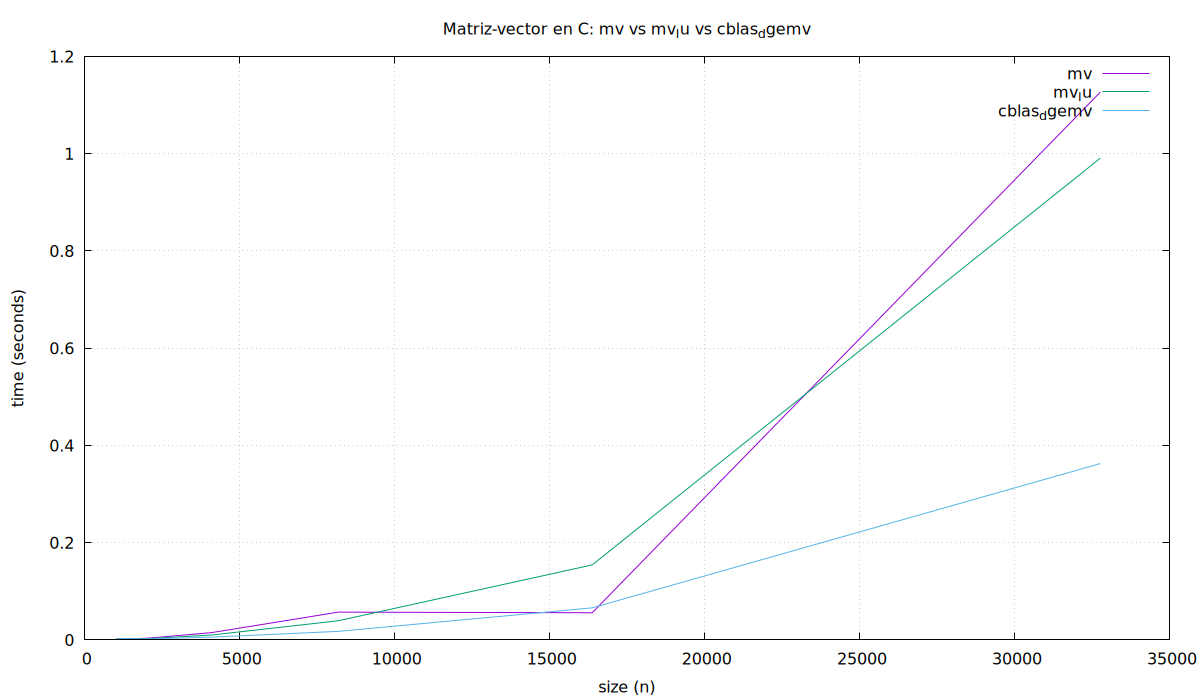
\includegraphics[width=0.9\textwidth]{c_mv_compare.png}
    \caption{Comparación entre multiplicación matriz-vector manual, optimizada y CBLAS.}
    \label{fig:c_mv_compare}
\end{figure}

\subsubsection{Multiplicación matriz-matriz}

\begin{table}[H]
\centering
\caption{Tiempos de ejecución para multiplicación matriz-matriz.}
\begin{tabular}{rrrr}
\toprule
$n$ & C manual & C optimizado & CBLAS \\
\midrule
128 & 0.00263500 & 0.000505571 & 0.00109614 \\
256 & 0.03306990 & 0.002533000 & 0.00257829 \\
512 & 0.81541800 & 0.018950000 & 0.00643086 \\
1024 & 7.14204000 & 0.162721000 & 0.02086140 \\
2048 & 174.15500000 & 2.759360000 & 0.06636690 \\
4096 & 4219.46000000 & 22.464200000 & 0.38605000 \\
\bottomrule
\end{tabular}
\end{table}

\begin{figure}[H]
    \centering
    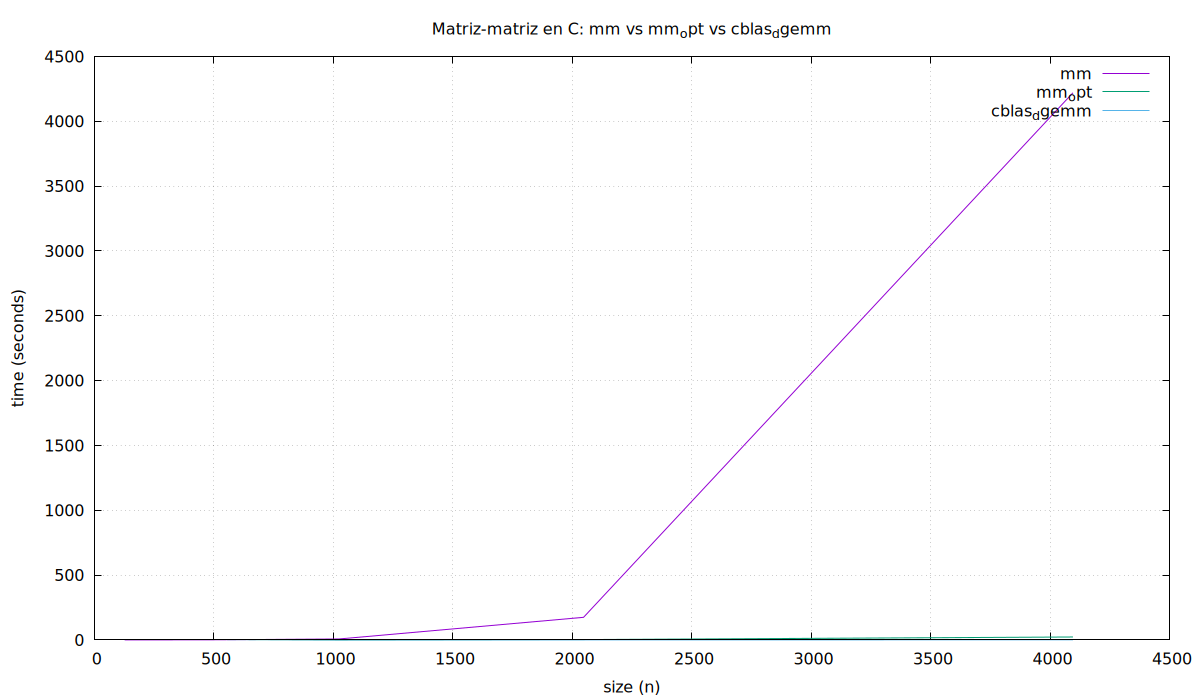
\includegraphics[width=0.9\textwidth]{c_mm_compare.png}
    \caption{Comparación entre multiplicación matriz-matriz manual, optimizada y CBLAS.}
    \label{fig:c_mm_compare}
\end{figure}

\begin{figure}[H]
    \centering
    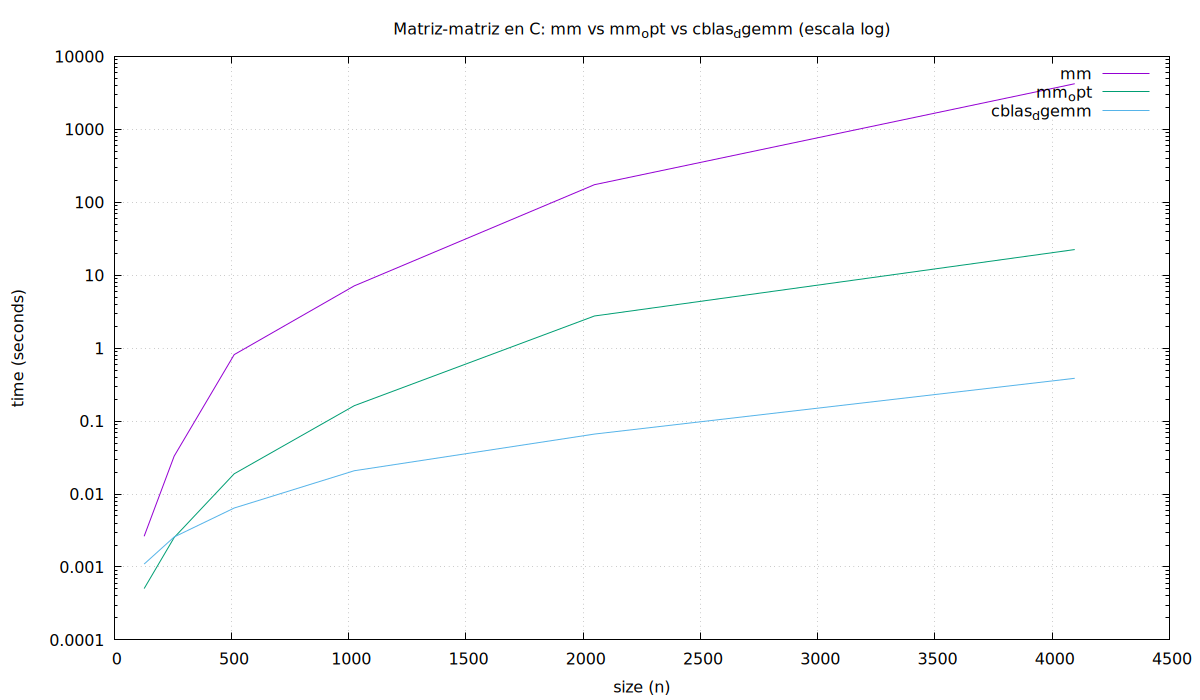
\includegraphics[width=0.9\textwidth]{c_mm_compare_log.png}
    \caption{Comparación matriz-matriz en escala logarítmica.}
    \label{fig:c_mm_compare_log}
\end{figure}

% =========================
% ANÁLISIS
% =========================
\section{Análisis de resultados}

\subsection{Análisis del producto punto}

El producto punto presentó un crecimiento aproximadamente lineal, coherente con su complejidad $O(n)$. En las implementaciones en C se observó que la versión optimizada mediante loop unrolling redujo el tiempo de ejecución en todos los tamaños evaluados.

Para tamaños pequeños, la función \texttt{cblas\_ddot} no siempre fue más rápida que las versiones manuales. Sin embargo, a medida que aumentó el tamaño del problema, CBLAS presentó mejores resultados. Esto se debe a que las rutinas BLAS están diseñadas para aprovechar mejor las características de la arquitectura y reducir costos de ejecución en problemas de mayor escala.

\subsection{Análisis de la multiplicación matriz-vector}

La multiplicación matriz-vector presentó un crecimiento superior al producto punto, lo que es coherente con su complejidad $O(n^2)$. La versión optimizada en C logró mejorar el rendimiento respecto a la versión manual en varios tamaños.

Sin embargo, se observó una medición irregular en el tamaño $n = 16384$, donde la versión optimizada presentó un tiempo mayor al esperado. Esta irregularidad puede estar asociada a ruido del sistema, carga del procesador, administración de memoria o efectos de caché. Por esta razón, dicho punto debe ser interpretado como una medición atípica y no como una tendencia general del algoritmo.

En tamaños grandes, CBLAS presentó un rendimiento superior, confirmando la ventaja de utilizar rutinas especializadas para operaciones de álgebra lineal.

\subsection{Análisis de la multiplicación matriz-matriz}

La multiplicación matriz-matriz fue la operación con mayor diferencia entre las implementaciones. La versión manual presentó tiempos muy elevados, especialmente para tamaños grandes. Esto se explica por su complejidad $O(n^3)$ y por el acceso menos eficiente a memoria.

La versión optimizada mediante cambio del orden de ciclos redujo considerablemente los tiempos de ejecución. En particular, para $n = 4096$, la versión manual tardó 4219.46 segundos, mientras que la versión optimizada tardó 22.4642 segundos. Esto demuestra el impacto de la localidad de memoria sobre el rendimiento.

A pesar de la mejora obtenida, \texttt{cblas\_dgemm} fue ampliamente superior, alcanzando 0.38605 segundos para el mismo tamaño. Este resultado evidencia el alto nivel de optimización de BLAS para operaciones matriciales.

% =========================
% DISCUSIÓN
% =========================
\section{Discusión}

Los resultados obtenidos permiten observar que la elección de la implementación influye directamente en el rendimiento. Aunque todos los algoritmos resuelven matemáticamente el mismo problema, sus tiempos de ejecución pueden variar de forma considerable.

En Octave, los operadores nativos fueron mucho más eficientes que las funciones implementadas manualmente con ciclos. Esto se debe a que las funciones escritas directamente en Octave son interpretadas, mientras que los operadores nativos suelen apoyarse en rutinas compiladas.

En C, las optimizaciones aplicadas permitieron mejorar el rendimiento de las versiones manuales. El loop unrolling fue útil en el producto punto y en la multiplicación matriz-vector. Sin embargo, la mejora más significativa ocurrió en la multiplicación matriz-matriz, donde el cambio en el orden de los ciclos permitió mejorar la localidad de memoria.

Finalmente, las funciones CBLAS demostraron el mejor rendimiento general. Esto se debe a que BLAS está diseñado específicamente para operaciones de álgebra lineal y aprovecha optimizaciones internas que son difíciles de igualar con implementaciones manuales simples.

% =========================
% CONCLUSIONES
% =========================
\section{Conclusiones}

A partir del desarrollo de la práctica, se concluye que la complejidad algorítmica tiene un impacto directo en el tiempo de ejecución. El producto punto presentó un crecimiento lineal, la multiplicación matriz-vector un crecimiento cuadrático y la multiplicación matriz-matriz un crecimiento cúbico.

Las implementaciones en C fueron considerablemente más rápidas que las funciones interpretadas en Octave. Además, las optimizaciones aplicadas permitieron reducir los tiempos de ejecución, especialmente en la multiplicación matriz-matriz.

La técnica de loop unrolling permitió mejorar el rendimiento en operaciones con ciclos internos simples. Por otra parte, el cambio en el orden de los ciclos tuvo un impacto mayor en la multiplicación matriz-matriz debido a la mejora en el acceso a memoria.

CBLAS obtuvo los mejores resultados en la mayoría de los casos, principalmente para tamaños grandes. Esto confirma que, cuando se trabaja con operaciones intensivas de álgebra lineal, es recomendable utilizar bibliotecas optimizadas en lugar de implementaciones manuales.

Finalmente, la práctica permitió comprobar experimentalmente la relación entre complejidad algorítmica, lenguaje de programación, optimización de código, acceso a memoria y rendimiento computacional.

% =========================
% ANEXOS
% =========================
\section{Anexos}

\subsection{Estructura de carpetas}

\begin{lstlisting}[language=bash]
practica1/
|-- octave/
|-- cblas/
|   |-- array/
|   |-- ddot/
|   |-- dgemv/
|   |-- dgemm/
|-- c/
|   |-- dot/
|   |-- mv/
|   |-- mm/
|-- resultados/
|   |-- datos/
|   |-- graficos/
|-- informe_latex/
\end{lstlisting}

\subsection{Código principal de producto punto en C}

\lstinputlisting[language=C]{../c/dot/dot.c}

\subsection{Código optimizado de producto punto en C}

\lstinputlisting[language=C]{../c/dot/dot_lu.c}

\subsection{Código principal de matriz-vector en C}

\lstinputlisting[language=C]{../c/mv/mv.c}

\subsection{Código optimizado de matriz-vector en C}

\lstinputlisting[language=C]{../c/mv/mv_lu.c}

\subsection{Código principal de matriz-matriz en C}

\lstinputlisting[language=C]{../c/mm/mm.c}

\subsection{Código optimizado de matriz-matriz en C}

\lstinputlisting[language=C]{../c/mm/mm_opt.c}

\subsection{Script de comparación para producto punto}

\lstinputlisting[language=bash]{../c/dot/dot_compare.sh}

\subsection{Script de comparación para matriz-vector}

\lstinputlisting[language=bash]{../c/mv/mv_compare.sh}

\subsection{Script de comparación para matriz-matriz}

\lstinputlisting[language=bash]{../c/mm/mm_compare.sh}

\end{document}
